\documentclass[]{article}
\usepackage{graphicx}
%opening
\title{Appunti di Automi e Linguaggi Formali}
\author{Nicola Baesso}

\begin{document}

	\maketitle
	
	\newpage
	\tableofcontents
	\newpage
	
	\textbf{Disclaimer}
	\newline
	\newline
	Questi appunti sono una raccolta parziale delle spiegazioni del prof. Bresolin, e sono state scritte con la gioia di poterle portare al primo parziale dell'anno. Si consiglia comunque di utilizzare solo come eventuale ripasso e non come testo di studio.
	\newpage
	\section{Introduzione}
		\subsection{Definizioni utili alla comprensione}
			Per questo corso, ci si avvarrà di alcune definizioni riportate in seguito, utili per una migliore comprensione della materia.
			\subsubsection{Algoritmi e Problemi}
				Un problema è definito da 3 (tre) caratteristiche specifiche: l'insieme dei possibili input, l'insieme dei possibili output e la relazione che collega questi due insiemi.
				\newline
				Un algoritmo è una procedura meccanica che, eseguendo delle computazioni eseguibili da un calcolatore, risolve un determinato problema se per ogni input si ferma dopo un numero finito di passaggi e produce un output corretto.
				\newline Inoltre è composto da una complessità temporale, che indica il tempo di esecuzione, e una complessità spaziale, che indica la quantità di memoria utilizzata. Entrambe queste misure sono dipendenti dalla dimensione dell'input.
			\subsubsection{Linguaggi formali}
				Un linguaggio formale può essere definito come un'astrazione del concetto di problema. 
				\newline
				Infatti, un problema può essere espresso sia come un insieme di stringhe (che da qui in avanti indicheremo con Linguaggio), con soluzioni che indicano se una stringa è presente nel Linguaggio o meno, oppure come una trasformazione tra vari Linguaggi, dove la soluzione trasforma una stringa di input in una stringa di output.
				\newline
				Quindi, ogni processo computazionale può essere ridotto ad una determinazione dell'appartenenza ad un insieme di stringhe, oppure essere ridotto ad una mappatura tra insiemi di stringhe.
			\subsubsection{Automi}
				Un automa è un dispositivo matematico (inteso in forma astratta) che può determinare l'appartenenza di una stringa ad un Linguaggio e può trasformare una stringa in una seconda stringa. Possiede ogni aspetto di un computer, poichè dato un input provvede a fornire un output, è dotato di memoria e ha la capacità di prendere delle decisioni.
				\newline
				La memoria per un automa è fondamentale. Sostanzialmente esistono automi a memoria finita e automi a memoria infinita, quest'ultimi con accesso limitato e non.
				\newline Chiaramente si hanno vari tipi di automi, ognuno di questi adatti ad una determinata classe di linguaggi, dove vengono differenziati per quantità di memoria e per il tipo di accesso ad essa.
			\subsubsection{Alfabeto e Linguaggio}
				Esattamente come nel caso del linguaggio naturale, un alfabeto è un insieme finito e non vuoto di simboli, ed è indicato con il simbolo $\Sigma$. Da esso si ha la stringa, ovvero una sequenza finita di simboli presi da un alfabeto. Inoltre, si definisce come stringa vuota la stringa senza alcun simbolo preso dall'alfabeto, e si indica con il simbolo $\varepsilon$. Infine la lunghezza di una stringa indica il numero di simboli presenti nella stringa, indicandola con \textbar w\textbar, con w una stringa qualsiasi .
				\newline
				\newline
				\textbf{Esempio}
				Si consideri il codice binario, composto da 0 ed 1. Allora definiremo l'alfabeto come $\Sigma$=\{0,1\}, una stringa valida come w=010110, e in questo particolare caso \textbar w\textbar=6.
				\newline
				\newline
				La potenza di un alfabeto, espressa come $\Sigma$$^k$ con k$\textgreater$0, esprime l'insieme delle stringhe composte da simboli dell'alfabeto di lunghezza k. L'espressione $\Sigma$$^*$ indica l'insieme di tutte le stringhe sull'alfabeto.
				\newline
				\newline
				\textbf{Esempio}
				Consideriamo nuovamente il codice binario. Per 0$\textless$k$\textless$2 (inclusi) si ha \newline
				$\Sigma$$^0$=$\varepsilon$ (la stringa vuota) \newline
				$\Sigma$$^1$=\{0,1\}\newline
				$\Sigma$$^2$=\{00,01,10,11\} \newline
				E così per ogni k positivo. Mentre $\Sigma$$^*$=$\Sigma$$^0$ $\cup$ $\Sigma$$^1$ $\cup$ $\Sigma$$^2$ \ldots \newline \newline 
				Quindi la potenza di un alfabeto crea a sua volta un alfabeto, con stringhe di lunghezza k, e tale alfabeto è composto da 2$^k$ stringhe. 
				\newline
				\newline
				Un linguaggio L è un sottoinsieme dell'insieme di tutte le stringhe dell'alfabeto. In simboli: L $\subseteq$ $\Sigma$$^*$ per un certo $\Sigma$.
	\section{DFA, NFA, espressioni e Linguaggi (non) regolari}
		Dopo aver appreso le definizioni necessarie, andiamo a scoprire in questa sezione i primi automi (DFA ed NFA), cosa sono le espressioni regolari e cosa sono i Linguaggi non Regolari.
		\subsection{DFA}
			Gli Automi a Stati Finiti (in Inglese Deterministic Finite Automation, abbreviato in DFA) sono la forma più semplice di automa e dispongono di una quantità finita di memoria.
			Tali automi accettano una parola nel linguaggio unicamente se è in uno stato terminale.
			\newline
			\newline
			\textbf{Esempio}
			Trovare ogni parola nel linguaggio binario che sia composta da un numero pari di 1.\newline
			Per creare questro DFA, abbiamo bisogno di due stati:\newline
			-Il primo sarà lo stato con il numero pari di 1. Tale stato sarà sia iniziale che terminale (e quindi accetterà la stringa).\newline
			-Il secondo sarà lo stato nel quale si ha un numero dispari di 1. In tale stato l'automa non accetterà la stringa.\newline
			Nel caso s'incontri uno 0, si deve rimanere nello stato attuale.\newline
			Segue il diagramma di transizione dell'automa, fatto con JFlap:
			\newline
			\begin{center}
				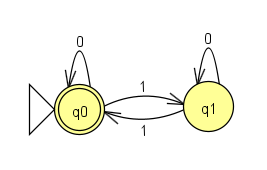
\includegraphics{DFA1.png}
			\end{center}
			Si noti, nel esempio, che ogni stato esegue una transizione \textbf{per ogni simbolo nel linguaggio}. Inoltre, quello che fa l'automa è semplicemente "contare" quante cifre di 1 sono presenti, accettando la stringa solo quando questa cifra è pari.\newline
			In generale, possiamo dire che un DFA utilizza un numero di stati per "contare" ad un determinato scopo, ed ha una transizione per ogni simbolo del linguaggio che deve analizzare.\newline
			\newline
			In maniera formale, un DFA si definisce con A=(Q,$\Sigma$,$\delta$,q0,F), dove Q è un insieme finito di stati, $\Sigma$ è un alfabeto finito (rappresenta i simboli dati in input al DFA), $\delta$ è una funzione di transizione ((q,a)$\mapsto$ q'), q0 è lo stato iniziale (e logicamente è nell'insieme di tutti gli stati dell'automa. In simboli: q0 $\in$ Q), e F è un insieme di stati finali (ovvero gli stati dove l'automa accetta la stringa, in simboli F $\subseteq$ Q).
			\newline
			\newline
			Come già visto nell'esempio, un DFA può essere graficamente rappresentato con cerchi, ad indicare gli stati, e con frecce, ad indicarne le transizioni. Però un DFA può essere rappresentato anche tramite una tabella, chiamata tabella di transizione.
			\newline
			\newline
			\textbf{Esempio} Riprendiamo l'esempio precedente. \newline
			Abbiamo già espresso l'automa che accetta ogni linguaggio con un numero pari di 1 come diagramma di transizione. Ora rappresentiamolo come tabella di transizione. \newline
			Per fare ciò, partiamo dallo stato iniziale, nel nostro caso q0, e ci segniamo le sue transizioni: se si ha uno 0, l'automa resta in q0, mentre se si ha un 1 l'automa va nello stato q1. Per q1 si fa la stessa cosa: se si ha uno 0, l'automa resta in q1, mentre con un 1 l'automa va (in questo caso, ritorna) in q0.\newline
			Di seguito, in forma tabellare, quel che ci siamo appena detti: \newline
			\begin{center}
				\begin{tabular}{c|c|c}
					 &0&1 \\
					 \hline
					$\rightarrow$ q0* &q0*&q1 \\
					q1&q1&q0*
				\end{tabular}
			\end{center}
			Come si nota dall'esempio, nella tabella di transizione si segna con una freccia lo stato iniziale dell'automa, e con un asterisco lo stato finale dell'automa stesso (che nel nostro esempio coincide con lo stato iniziale, ma non è sempre così).\newline
			\textbf{Importante!} Un DFA accetta una parola w se la sua computazione accetta w, ovvero l'automa termina in uno stato finale. Inoltre, se il DFA accetta w, allora w appartiene ad un linguaggio regolare. \newline
			Più formalmente, si indica con L(A)=\{w $\in$ $\Sigma$$^*$  \textbar A accetta w\} il linguaggio accettato, che è un linguaggio regolare.
		\subsection{NFA}
			Gli Automi a Stati Finiti non Deterministici (in inglese Nondeterministic Finite Automation, abbreviato in NFA) sono una forma di automi a stati finiti, che è utilizzato in contesti dove "contare" non è semplice, quindi si lascia spazio al non-determinismo. \newline
			\textbf{Esempio} Costruire un NFA che riconosca la parola che, sull'alfabeto \{a,b,c\}, non sia composto da tutti i simboli. \newline
			Per questo esempio, usare un DFA risulterebbe alquanto complesso, quindi ci avvarremo di un NFA per semplicità. Infatti, ci saranno sufficienti 4 stati e 6 transizioni in tutto. Di seguito troviamo sia tabella che diagramma di transizione per il seguente NFA:\newline
			\begin{center}
				\begin{tabular}{c|c|c|c}
					&a&b&c \\
					\hline
					$\rightarrow$ q0 &\{q1,q3\}*&\{q1,q2\}*&\{q2,q3\}* \\
					\{q1,q2\}* &q1*&\{q1,q2\}*&q2* \\
					\{q1,q3\}* &\{q1,q3\}*&q1*&q3* \\
					\{q2,q3\}* &q3*&q2*&\{q2,q3\}* \\
					q1* &q1*&q1*&$\emptyset$ \\
					q2* &$\emptyset$&q2*&q2* \\
					q3* &q3*&$\emptyset$&q3* \\
				\end{tabular}
			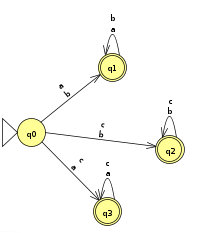
\includegraphics{NFA1.png}
			\end{center}
			Esattamente come prima, nella tabella rappresentiamo lo stato iniziale con una freccia e con un asterisco rappresentiamo lo stato finale. Generalmente, può capitare che la tabella di transizione può essere "smagrita" ovvero che la tabella completa contiene transizioni a stati mai attraversati dall'automa (non è il caso dell'esempio), e quindi possono essere rimossi. Notiamo però che gli stati inclusi nella tabella non sono semplicemente solo gli stati semplici ma includo anche dei "gruppi" di stati, essendo le transizioni dirette in più stati (grazie al non-determinismo).\newline
			Formalizziamo: un NFA NA è descritto con NA=(Q,$\Sigma$,$\delta$,q0,F), con l'unica differenza (rispetto ai DFA) che la funzione di transizione restituisce un sottoinsieme di Q. \newline
			\textbf{Importante!} Un NFA, a differenza di un DFA, può non arrivare alla fine della computazione ed interrompersi prima (come si nota bene dalle tabelle di transizioni), e quindi accetta una parola w se almeno una sua computazione accetta w, ovvero l'automa termina, in almeno una delle sue computazioni, in uno stato finale. Esattamente come nel DFA, se l'NFA accetta w, allora w appartiene ad un linguaggio regolare (la formalizzazione è la stessa).
			\subsubsection{$\varepsilon$-NFA}
				Gli $\varepsilon$-NFA sono NFA che utilizzano le $\varepsilon$-transizioni, ovvero utilizza transizioni che \textbf{non consumano il carattere}, quindi l'automa passa allo stato successivo mantenendo la stringa come prima. \newline
				\textbf{Esempio} Costruire un $\varepsilon$-NFA che accetti numeri decimali, riconoscendo il segno (opzionale),una stringa di decimali, un punto e un altra stringa di decimali, tenendo conto che una delle stringhe di decimali non può essere vuota. \newline
				In questo caso, usare un NFA semplice non è una buona idea, poichè non ci permette di dare opzionalità per quanto riguarda il segno. Inoltre non ci farebbe finire in uno stato finale al termine della lettura dei decimali. Di seguito troviamo sia tabella che diagramma di transizione per il seguente $\varepsilon$-NFA:\newline
				\begin{center}
					\begin{tabular}{c|c|c|c|c}
						&$\varepsilon$&+,-&.&0,..,9 \\
						\hline
						$\rightarrow$ q0 &q1&q1&$\emptyset$&$\emptyset$ \\
						q1 &$\emptyset$&$\emptyset$&q2&\{q1,q4\} \\
						q2 &$\emptyset$&$\emptyset$&$\emptyset$&q3 \\
						q3 &q5*&$\emptyset$&$\emptyset$&q3 \\
						q4 &$\emptyset$&$\emptyset$&q3&$\emptyset$ \\
						q5* &$\emptyset$&$\emptyset$&$\emptyset$&$\emptyset$
					\end{tabular}
					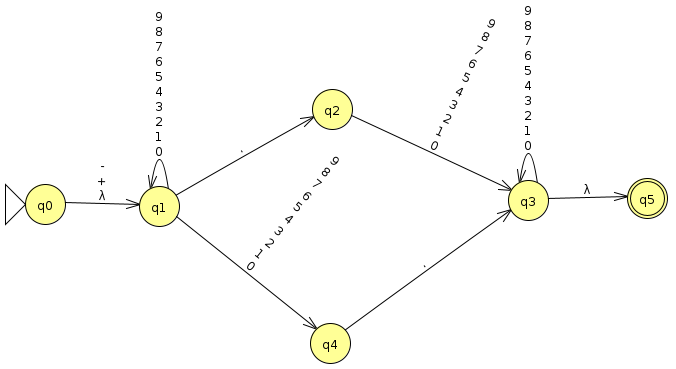
\includegraphics[scale=0.7]{e-NFA1.png}
				\end{center}
				Essendo lo stato \{q1,q4\} non raggiungibile, si omette nella tabella.\newline
				Formalmente, un $\varepsilon$-NFA E è definito come E=(Q,$\Sigma$,$\delta$,q0,F), dove l'unico parametro differente è la funzione di transizione, che prende in input uno stato in Q e un simbolo nell'alfabeto $\Sigma$$\cup$\{$\varepsilon$\}, restituendo un sottoinsieme di Q. \newline
				Essendo un particolare tipo di NFA, l'$\varepsilon$-NFA ha tutte le caratteristiche degli NFA.
		\subsection{DFA to NFA (e viceversa)}
			Sebbene possa sembrare controintuitivo, sia NFA che DFA riconoscono gli stessi linguaggi cambiando unicamente il metodo con cui li riconoscono.\newline Infatti, $\forall$ NFA N $\exists$ un DFA D : L(D)=L(N) (e viceversa). Per far ciò, si usa un metodo chiamato Costruzione a Sottoinsiemi.
			\subsubsection{Costruzione a Sottoinsiemi}
				La Costruzione a Sottoinsiemi ci permette, dato un NFA, di ricavare un DFA che possa riconoscere il linguaggio del NFA. In particolare, ogni stato del DFA corrisponde ad un insieme di stati del NFA, il DFA inizia in \{q0\}, ovvero nell'insieme di stati con solo q0, nel DFA una stato finale corrisponde ad almeno uno stato finale del NFA, e la funzione di transizione del DFA si riferisce ad uno stato contenuto nel target della funzione di transizione di un NFA.\newline \newline
				\textbf{Esempio} Prendiamo il seguente NFA:
				\begin{center}
					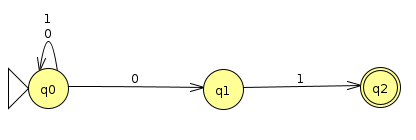
\includegraphics{NFADFA1.png}
				\end{center}
				Per "tradurlo" in un DFA, dobbiamo fare una tabella di "conversione", come la seguente:
				\begin{center}
					\begin{tabular}{c|c|c}
						&0&1 \\
						\hline
						$\rightarrow$ \{q0\} &\{q0,q1\}&\{q0\} \\
						\{q1\} &$\emptyset$&\{q2\}* \\
						\{q2\}* &$\emptyset$&$\emptyset$ \\
						\{q0,q1\} &\{q0,q1\}&\{q0,q1,q2\}* \\
						\{q0,q2\}* &\{q0,q1\}&\{q0,q1\} \\
						\{q1,q2\}*&$\emptyset$&\{q2\}*\\
						\{q0,q1,q2\}* &\{q0,q1\}&\{q0,q1,q2\}* 
					\end{tabular}
				\end{center}
				Ma se osserviamo, alcuni stati sono inutili, ovvero non contribuiscono in alcun modo alla creazione del DFA, e l'automa non passerà mai per quei stati. Se "puliamo" la tabella otteniamo:
				\begin{center}
					\begin{tabular}{c|c|c}
						&0&1 \\
						\hline
						$\rightarrow$ \{q0\} &\{q0,q1\}&\{q0\} \\
						\{q0,q1\} &\{q0,q1\}&\{q0,q1,q2\}* \\
						\{q0,q1,q2\}* &\{q0,q1\}&\{q0,q1,q2\}* 
					\end{tabular}
				\end{center}
				Che comprende gli stati che formano realmente il DFA. Se costruiamo il diagramma otteniamo:
				\begin{center}
					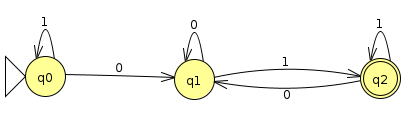
\includegraphics{NFADFA2.png}
				\end{center}
				Che è effettivamente corrispondente agli stati e alle transizioni della seconda tabella.\newline
				Tale operazione è possibile grazie ad un teorema, che ora enunciamo.
				\newline \newline
				\textbf{Teorema di equivalenza}\newline
				Un linguaggio L è accettato da un DFA $\Leftrightarrow$ L è accettato da un NFA
			\subsubsection{$\varepsilon$-chiusure}
				Nel caso di $\varepsilon$-NFA, si utilizza una versione modificata della costruzione a sottoinsiemi, caratterizzata dalle $\varepsilon$-chiusure. Con $\varepsilon$-chiusura s'intende l'eliminazione delle $\varepsilon$-transizioni dagli stati che ne fanno uso.\newline
				A livello pratico. la costruzione a sottoinsiemi è uguale a quella usata partendo da un NFA, con la variante che lo stato iniziale del DFA è dato dalle $\varepsilon$-chiusure dello stato iniziale del $\varepsilon$-NFA.
				\newline \newline
				\textbf{Esempio} Riprendiamo l'$\varepsilon$-NFA visto in precedenza:
				\begin{center}
					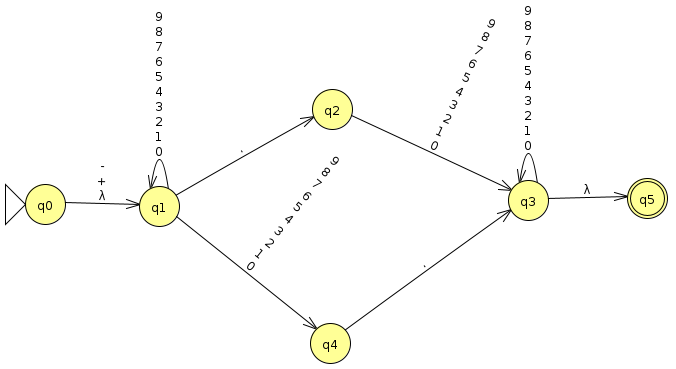
\includegraphics[scale=0.7]{e-NFA1.png}
				\end{center}
				Prima di effettuare la costruzione, dobbiamo effettuare le $\varepsilon$-chiusure: \newline \\
				ECLOSE(q0)=\{q0,q1\}\\
				ECLOSE(q1)=\{q1\}\\
				ECLOSE(q2)=\{q2\}\\
				ECLOSE(q3)=\{q3,q5\}\\
				ECLOSE(q4)=\{q4\}\\
				ECLOSE(q5)=\{q5\}\\
				Dopo questa operazione, possiamo applicare la costruzione. Riportiamo solo la tabella di transizione (per pigrizia):
				\begin{center}
					\begin{tabular}{c|c|c|c}
						&+,-&.&0,..,9 \\
						\hline
						$\rightarrow$ \{q0,q1\} &\{q1\}&\{q2\}&\{q1,q4\} \\
						\{q1\} &$\emptyset$&\{q2\}&\{q1,q4\} \\
						\{q2\} &$\emptyset$&$\emptyset$&\{q3,q5\}* \\
						\{q1,q4\} &$\emptyset$&\{q2,q3,q5\}&\{q1,q4\} \\
						\{q2,q3,q5\}* &$\emptyset$&$\emptyset$&\{q2.q3,q5\} \\
						\{q3,q5\}* &$\emptyset$&$\emptyset$&\{q3,q5\} \\
					\end{tabular}
				\end{center}
				Enunciamo ancheil teorema per la conversione da $\varepsilon$-NFA a DFA:
				\newline
				\newline
				\textbf{Teorema}\newline
				Un linguaggio L è accettato da un DFA $\Leftrightarrow$ L è accettato da un $\varepsilon$-NFA
	\section{Grammatiche di Linguaggi liberi da contesto e PDA}
\end{document}
